\cotefile{91}
\scanpage{59}
% archive foliation: 58
\unsure{comme pour}
\[
T\longrightarrow f_*^{\text{ét}.}(T)
\]
qui est \unsure{tel} que l'hom canonique
\[
\underline{\mathrm{Hom}}_S(\overbrace{f_*^{\text{ét}}(T)}^{\inserted{\overline T}},S')\longrightarrow
\underline{\mathrm{Hom}}_S(T,S')
\]
est un isom. pour tt $S'$. (\unsure{raison} --). Il en résulte que pour tt \deleted{\unsure{$S'\to S$}} changement de base
\deleted{$\underline{\mathrm{Hom}}_{\overline{k(s)}}(\overline T_{\bar s},S'_{\bar s})\to$}
(\unsure{p. ex.} $\bar s=\operatorname{Spec}(\overline{k(s)})$)
la \deleted{\unsure{a}} relation reste vraie; faisant $S'=S\times I$ ($I$ \unsure{un fini}) on en conclut que
$T\to f_*^{\text{ét}}(T)$ est surjectif et \inserted{(si $T/S$ est fini)} géométriquement injectif
(\unsure{regarder} \deleted{\unsure{un}} \inserted{un ensemble} \unsure{ch.} pour tt $s\in S$).

Inversement, si $T\to\overline T$ est un morphisme surjectif et géom. injectif de $T$ (fini \inserted{et plat} sur $S$) sur $\overline T$ \unsure{sch.} étale de $S$, alors on a
\[
\underline{\mathrm{Hom}}_S(\overline T,S')=\mathrm{Hom}_S(T,S')
\]
pour tout $S'$ non ramifié sur $S$ (\unsure{enfin} $\unsure{f}$ est \unsure{comme} \unsure{le} $=$ \unsure{dessus} reste vrai par \unsure{chgt.} de la base\inserted{$(S)$}),
\unsure{encore} \deleted{\unsure{$\mathrm{H}$}}
$\underline{\mathrm{Hom}}_S(\overline T,S')\simeq\underline{\mathrm{Hom}}_S(T,S')$,
\unsure{isom.} \unsure{T---}.

\scanpage{61}
\textcircled{1}
% archive foliation: 60
\uline{\unsure{Set up} général}

Soit $S$ un préschéma. \deleted{\unsure{Algèbre}\illegible{2}}

Soit $\underline W$ un foncteur covariant de la catégorie des $S$-préschémas dans la catégorie des \deleted{\unsure{$S$}} préschémas. On suppose $\underline W$ ``de nature locale'', i.e.

a i) Si $i:T\to T'$ est une immersion ouverte, alors $\underline W(i):\underline W(T)\to\underline W(T')$ est une immersion ouverte.
[Donc si $U$ ouvert dans $T$, on identifie $\underline W(U)$ à un ouvert de $\underline W(T)$]

\margin{\unsure{on fera} cette hypothèse \unsure{de suite} \deleted{\unsure{tt}}}

a ii)
\[
\underline W(\bigcup U_i)=\bigcup_i\underline W(U_i)
\]
pour une réunion \unsure{quelc.} de parties ouvertes de $T$

a iii)
\[
\underline W(U\cap V)=\underline W(U)\cap\underline W(V)
\]

\uline{Exemple I}. Soit $S'$ un $S$-préschéma. Posons $\underline W_{S'}(T)=T\times_S S'$; on obtient ainsi \inserted{$\underline W_{S'}$} un foncteur covariant de nature locale des $S$-préschémas dans les $S'$-préschémas (a fortiori dans les préschémas).

\inserted{Cas $\mathrm I'$ : $S'$ est fini et loc. libre sur $S$}

\uline{Exemple II} Soit $W$ un \deleted{\unsure{$S$}} préschéma en anneaux commutatifs sur $S$, supposons que pour tt $T/S$, le faisceau d'anneaux $\underline\Gamma(W_T/T)$ sur $T$ fasse de $T$ un \figure{\begin{tikzpicture}[baseline=(p.base)]\node[draw,ellipse,inner sep=3pt] (p) {\unsure{préschéma}};\end{tikzpicture}} (cf exemple plus bas), \deleted{\unsure{le} \illegible{1} \unsure{ainsi}}
\margin{\unsure{associé aux} \unsure{anneaux locaux}}

\scanpage{62}
% archive foliation: 61
\deleted{\unsure{un foncteur}}
et que l'hom naturel $\underline\Gamma(W_T/T)\to\underline\Gamma(W_{T'}/T')$ pour $T'\to T$ \deleted{\unsure{défini}} soit \uline{local} sur les fibres des faisceaux. On obtient ainsi un foncteur \inserted{$\underline W$} de nature \unsure{covar.} des $S$-préschémas en $S$-préschémas, et un isom fonctoriel
\[
|\underline W(T)|\simeq|T|\quad\text{(espaces ss-jacents)}.
\]
\deleted{\unsure{Nous donnerons des} \unsure{préschémas} d'anneaux $\Lambda$, \unsure{puis que} \illegible{2} $\mathrm{Hom}_S(T,\Lambda)=$ \unsure{conditions} suffisantes plus bas pour que $\Lambda$ ait les \unsure{prop.} \unsure{voulues}.}

\uline{Exemple \unsure{III}} Soit $S'=\operatorname{Spec}(\mathcal A)$, où $\mathcal A$ est un faisceau loc. libre d'\unsure{algèbres} comm. sur $\underline O_S$. Supposons de plus que $S'\to S$ soit un homéomorphisme universel. Posons
$\Lambda=\deleted{\unsure{W}}\mathbf V(\check{\mathcal A})$.
On est alors simultanément dans le cas de l'exemple I et de l'exemple II.
\margin{$S'\to S$}

\inserted{\uline{Exemple \unsure{III'}} Comme II, mais on suppose donné une augmentation $W\to S[t]$ d'anneaux, telle que pour tout $T/S$ l'augmentation correspondante $\underline O_{\underline W(T)}\to\underline O_T$ soit surjective, de noyau nilpotent.}
\margin{\unsure{blague sur} exemple II : foncteurs de Greenberg}

Soit $\mathfrak X$ un préschéma sur $\underline W(S)$. Considérons le foncteur contravariant en le $S$-préschéma $T$
\[
(\ast)\qquad \mathrm{Hom}_{\underline W(S)}(\underline W(T),\mathfrak X)
\]

\scanpage{63}
% archive foliation: 62
On \deleted{\unsure{veut}} se demande s'il est représentable, i.e. on demande la valeur en $\unsure{T}$ du \uline{foncteur adjoint} (au sens de Kan) du foncteur $\underline W$ des $S$-préschémas en $\unsure{T}$-préschémas. Une solution du Pb concret posé par le foncteur en $T$ ci-dessus est par définition un couple
\[
X\quad\text{($S$-préschéma.)}\qquad \underline W(X)\xrightarrow{\alpha}\mathfrak X
\]
tel que pour tout $T$, l'application naturelle
\[
\mathrm{Hom}_S(T,X)\xrightarrow{\sim}\mathrm{Hom}_{\underline W(S)}(\underline W(T),\mathfrak X)
\]
\deleted{soit un} définie par \unsure{factorisation}
\diagram{\begin{tikzcd}[ampersand replacement=\&]
\underline W(T)\arrow[r,"\underline W(u)"]\&\underline W(X)\arrow[r,"\alpha"]\&\mathfrak X
\end{tikzcd}}
soit \uline{bijective}. Comme le foncteur $(\ast)$ en $T$ est de ``nature locale'', il suffit d'ailleurs de vérifier la bijectivité pour $T$ affine \deleted{\unsure{à}} \inserted{sur un ouvert} affine de $S$, p. ex.

Désignons par $\underline W^a$ le foncteur adjoint de $\underline W$ (défini sur une ss-catégorie de la catégorie des $\unsure{T}$-préschémas)
\margin{$\mathrm{Hom}_{S^a}(T^a,\mathfrak X)\simeq\mathrm{Hom}_S(T,\mathfrak X$}

\scanpage{64}
% archive foliation: 63
(i) Si $\underline W^a(\mathfrak X)$ et $\underline W^a(\mathfrak Y)$ sont définis, il en est de $=$ de $W^a(\mathfrak X\times_{W(S)}\mathfrak Y)$, et on a
\[
W^a(\mathfrak X\times_{W(S)}\mathfrak Y)\simeq
W^a(\mathfrak X)\times_S W^a(\mathfrak Y)
\]
et on a plus généralement \deleted{\unsure{pour}} les formules analogues pour les limites projectives finies [donc $(\alpha)$ l'objet unité $(\beta)$ les produits fibrés, d'où comme conséquences $(\gamma)$ Noyaux]

(ii)
\[
W^a(\mathfrak X)\times_S T\simeq W_T^a(\mathfrak X\times_{W(S)}W(T))
\]
[l'\unsure{existence} du premier mb implique celle du second; la définition de $W_T$ est claire --]

De (i) résulte que le foncteur $W^a$ transforme un préschéma en groupes, anneaux etc en préschéma de $=$ type.

\scanpage{65}
% archive foliation: 64
\uline{Supposons} que $W^a(W(S)[t])$ existe. C'est alors de façon naturelle un préschéma en anneaux sur $S$, que nous noterons $W$, appelé \uline{préschéma d'anneaux générateur du foncteur} $W$.

[Dans l'exemple II, c'est le schéma d'anneaux $W$ de départ. Dans le cas de l'exemple I, \deleted{c'est le} si \deleted{schéma} on suppose $S'$ \inserted{fini et} loc. libre sur $S$, c'est le \deleted{\unsure{faisc.}} schéma en anneaux $V(\check{\underline A})$, où $\underline A$ est le faisceau d'algèbres sur $S$ associé à $S'$].

Soit alors $\mathfrak X$ ss-schéma fermé de $W(S)[t_1,\ldots,t_r]$ défini par \deleted{\unsure{un}} le faisceau d'idéaux \deleted{\unsure{de}} $\underline O_{W(S)}[t_1,\ldots,t_r]$ engendré par des sections $F_i$ $(i=1,\ldots s)$, donc $\mathfrak X$ est le produit fibré, sur $\mathfrak Y^s$, de $\mathfrak Y^r$ et $\mathfrak Y^0$ [où $\mathfrak Y^{\deleted{\unsure{*}}}=W(S)[t]$].

\scanpage{66}
% archive foliation: 65
Alors $W^a(\mathfrak X)$ existe, et est aussi donné comme produit fibré. De façon précise, les $F_j$ \inserted{$(1\leq j\leq s)$} définissent des polynômes \unsure{avec} les $t_i$ $(1\leq i\leq r)$, à coefficients dans $\Gamma(\Lambda/S)$; d'où \deleted{\unsure{donc}} un $S$-morphisme $\Lambda^r\to\Lambda^s$, et $W^a(\mathfrak X)$ est $\simeq$ l'image inverse de la section nulle de $\Lambda^s$.

\uline{Exemples} \deleted{$\unsure{\mathfrak Y_r}$} $(G_{a\,\underline W(S)})^n$, $\mathrm{GL}(n)_{\underline W(S)}$, etc.

Soit $\underline W'(T)\xrightarrow{\unsure{\alpha(T)}}\underline W^{\deleted{\unsure{*}}}(T)$ un morphisme fonctoriel de préschémas, définissant en particulier
\[
\underline W'(S)\unsure{-|\to}\underline W(S)
\]
Soit de plus $\mathfrak X$ sur $W(S)$, posons
\[
\mathfrak X'=\mathfrak X\times_{\underline W(S)}\underline W'(S)
\]
On a alors, pour tout $T$, un hom
\margin{\deleted{\unsure{qui est d'ailleurs}}}
\[
(\ast)\quad \mathrm{Hom}_{\underline W(S)}(\underline W(T),\mathfrak X)\longrightarrow
\mathrm{Hom}_{\underline W'(S)}(\underline W(T)\times_{\underline W(S)}\underline W'(S),\mathfrak X')
\]
[image réciproque d'un morphisme par $W'(S)\unsure{-|\to}W(S)$]

d'autre part on a
\[
W'(T)\longrightarrow W(T)\times_{W(S)}W'(S)
\]
\deleted{par suite} qui a pour composantes $\underline W'(T)\unsure{-|\to}\deleted{\unsure{W}}\underline W(T)$ et $W'(T)\to W'(S)$, d'où
\[
(\ast\ast)\quad\mathrm{Hom}_{W'(S)}(W(T)\times_{W(S)}W'(S),\mathfrak X')\longrightarrow
\mathrm{Hom}_{W'(S)}(W'(T),\mathfrak X'\unsure{)}
\]
d'où en composant $(\ast)$ et $(\ast\ast)$ un \deleted{\unsure{hom}} \inserted{morphisme}, évidemment fonctoriel en $T$
\[
\mathrm{Hom}_{W(S)}(W(T),\mathfrak X)\longrightarrow\mathrm{Hom}_{W'(S)}(W'(T),\mathfrak X')
\]
Par suite, si $W^a(\mathfrak X)$ et $W'^a(\mathfrak X')$ existent, on a un morphisme canonique
\[
W^a(\mathfrak X)\xrightarrow{\alpha^*(\mathfrak X)}W'^a(\mathfrak X\deleted{\unsure{')|)}}\times_{W(S)}W'(S))
\]

\scanpage{67}
% archive foliation: 66
De cette façon, pour $\underline W$ fixé, \deleted{\unsure{$\mathfrak X$ fixé}} \deleted{\unsure{fixé}} $\mathfrak X$ et $W'$ variables,
\[
W'^a(\mathfrak X\times_{W(S)}W'(S)),
\]
devient un \uline{bifoncteur} en $\mathfrak X$, $W'$, \uline{covariant} en $\mathfrak X$, \uline{contravariant en} $W'$.

\textcircled{2} \uline{Critère d'existence : Cas affine}
\margin{Ici, il suffit que $W$ \unsure{en plus} transforme affines en affines \deleted{\unsure{sur un}}}
\margin{Foncteurs $W$ \uline{spécial} [\unsure{associé à un} schéma \deleted{\unsure{d'}} en anneaux sur $S$, affine sur $S$]}

Supposons que $\underline W$ transforme schémas affines (sur ouverts affines de $S$) en schémas affines. Donc, au dessus d'un ouvert affine de $S$, d'anneau $A$, $\underline W$ est défini par un foncteur covariant, également noté $\underline W$, des \unsure{fais.} $A$-algèbres \inserted{$B$} en anneaux $\underline W(B)$. [\unsure{Avec} l'hypothèse de \deleted{localité} \inserted{\unsure{caractère local}} de ce foncteur, que nous n'expliciterons pas]. On suppose qu'on a
\inserted{$\underline W(B)=\mathrm{Hom}_{A\text{-alg.}}(\Lambda,B)$}
où $\Lambda$ est \deleted{l'algèbre affine} \inserted{l'anneau} d'un schéma en anneaux \deleted{affine} sur $S$, affine sur $S$.

\scanpage{68}
% archive foliation: 67
[Cela est le cas en particulier dans le cas de l'exemple I, \deleted{$S'$ est} \inserted{lorsque $S'$ est} fini et loc. libre sur $S$, et l'exemple II, \inserted{lorsque} $W$ \deleted{\unsure{est}} est affine sur $S$].

\uline{Proposition} Dans ces conditions, si \deleted{$\mathfrak X$ est} $\mathfrak X$ est un schéma \uline{affine} sur $\underline W(S)$, $W^a(\mathfrak X)$ existe et est un schéma \uline{affine} sur $S$.

\uline{Démonstration} \deleted{\unsure{Soit}\ $\mathfrak X$} \inserted{On peut supposer $S$ affine.} Si $\mathfrak X=\operatorname{Spec}(\unsure{C})$ où $\unsure{C}$ est une algèbre de type fini \deleted{de} sur $\underline W(A)$, engendrée par $r$ éléments, il résulte de suite du \unsure{\S\ N° 1} que $W^a(\mathfrak X)$ existe et est $\simeq$ un sous-préschéma fermé de $W^r$ [défini par des ``équations algébriques'' à coeffs. \inserted{de} dans $\Gamma(W/S)$]. Comme $W$ est affine, il en est de $=$ de \deleted{$\unsure{W^r}$} $W^r$ donc aussi de $W^a(\mathfrak X)$ (\unsure{cqf}). On obtient d'ailleurs

\uline{Cor.} \deleted{Si \unsure{S aff.}\ \unsure{l\textquotesingle anneau de}} \inserted{Supposons $S$ affine.} Si $\unsure{\ell|C}$ est engendré par $r$ générateurs sur celui de $W(S)$, et celui de $W$ par $\unsure{v}$ génér. sur celui de $S$, alors

\scanpage{69}
% archive foliation: 68
l'anneau de $\underline W^a(\mathfrak X)$ est engendré par $\unsure{v}r$ générateurs sur celui de $S$.

Dans le cas général \inserted{($S$ affine)}, on a $C=\varinjlim C_i$, où les $C_i$ sont des ss-$W(A)$-algèbres \inserted{de type fini} de $C$. On a donc, pour $T$ affine
% The written argument order and the curved transposition stroke are both retained.
\[
\begin{aligned}
\mathrm{Hom}_{\underline W(S)}\text{\figure{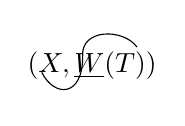
\begin{tikzpicture}[baseline=(args.base)]
\node[inner sep=0pt] (args) {$(\mathfrak X,\underline W(T))$};
\draw (-.64,-.08) .. controls (-.48,-.40) and (-.12,-.40) .. (-.12,.12) .. controls (-.15,.48) and (.40,.48) .. (.57,.24);
\end{tikzpicture}}}
&=\mathrm{Hom}_{W(A)\text{-alg}}(\deleted{\unsure{W(B)}}C,\underline W(B))\\
&\simeq\varprojlim\mathrm{Hom}_{\underline W(A)\text{-alg}}(C_i,\underline W(B))\\
&\simeq\varprojlim\mathrm{Hom}_{A\text{-alg}}(\underline W^a(C_i),B)\\
&\simeq\mathrm{Hom}_{A\text{-alg}}(\varinjlim\underline W^a(C_i),B)
\end{aligned}
\]
Soit donc
\[
\varinjlim W^a(C_i)=\deleted{\unsure{W^a}}D\qquad\deleted{\unsure{\longrightarrow}}
\]
on a obtenu un isom fonctoriel
\[
\mathrm{Hom}_{\underline W(S)}(\underline W(T),\mathfrak X)\simeq\mathrm{Hom}_S(T,\operatorname{Spec}(D)),
\]
d'où le résultat.

\inserted{\uline{Corollaire} Dans les conditions précédentes, si $\mathfrak X\xrightarrow{f}\mathfrak Y$ est un morphisme \deleted{affine} de $S$-préschémas affines qui est de type fini (resp. une immersion fermée)}
\margin{alors $\underline W^a(f)$ est un morphisme \uline{affine} de type fini pourvu que $W/S$ \unsure{soit} de type fini. resp. une immersion fermée}

\deleted{\uline{Corollaire} Soit $f:\mathfrak X\to\mathfrak Y$ un morphisme de $\underline W(S)$-préschémas, $\unsure{S}$ supposons que $\underline W^a(\mathfrak X)$ et $\underline W^a(\mathfrak Y)$ existent, alors $W$ $W^a(f):W^a(\mathfrak X)\unsure{-|\to}W^a(\mathfrak Y)$ est affine,}

\scanpage{70}
% archive foliation: 69
\textcircled{3} \uline{Recollement}

Aucune hypothèse sur $\underline W$

\deleted{\uline{Proposition}} \inserted{Lemme 1}
Soit $\mathfrak X$ sur $\underline W(S)$,
\deleted{$(\mathcal U_i)_{i\in I}$ une famille d'ouverts sur $\mathfrak X$. On suppose que pour tout $T$ sur $S$, et \deleted{$\underline W(T)$ est réunion} \deleted{tout} \inserted{$\underline W(S)$-}morphisme $\underline W(T)\xrightarrow{f}\mathfrak X$, on a $T=\bigcup T_i$ (les $T_i$ ouverts), avec $f(\underline W(T_i))\subset\mathfrak X_i$. Si les $W^a$}
$\mathcal U$ un ouvert de $\mathfrak X$, on suppose que $\underline W^a(\mathfrak X)=X$ existe, soit $\mathcal U'$ l'image inverse de $\mathcal U$ par
\diagram{\begin{tikzcd}[ampersand replacement=\&]
\underline W(X)\arrow[r,"\varphi"]\&\mathfrak X\\
\mathcal U'\arrow[u,phantom,"\cup" description]\&\mathcal U\arrow[u,phantom,"\cup" description]
\end{tikzcd}}

Supposons : \textcircled{$\alpha$} qu'il existe un ouvert $U$ de $X$ tel que pour tout $T/S$, et tout morphisme $\underline W(T)\xrightarrow{f}\underline W(X)$, la condition
\[
f(\underline W(T))\subset\mathcal U'\Longleftrightarrow f(\underline W(T))\subset\underline W(U)
\]
[En particulier, on a $W(U)\subset\mathcal U'$]
Dans ces conditions, $U$ muni du morphisme $W(U)\to\mathcal U$ induit par $\underline W(X)\to X$ est un $W(\unsure{\mathcal U'|\mathcal U})$.

\scanpage{71}
% archive foliation: 70
C'est trivial.

\deleted{Cas particuliers\quad \uline{Proposition} Dans les cas des $\unsure{\mathrm I'}$ ou $\unsure{\mathrm{II}''}$, si $W^a(\mathfrak X)$ existe et}

\uline{Lemme 2} Soient $\mathfrak X_i$ des ouverts de $\mathfrak X/W(S)$, on suppose \deleted{que $\underline W^a(\mathfrak X)$ existe} que \deleted{les $\mathfrak X_i$ dans $\mathfrak X$ \unsure{vérifient} les conditions du Lemme 1 (en particulier} les $W^a(\mathfrak X_i)$ existent \deleted{et que} \deleted{)} et que les $\mathfrak X_i\cap\mathfrak X_j$ dans $\mathfrak X_i$ satisfont les $=$ conditions \inserted{du lemme 1}, [donc $\underline W^a(\mathfrak X_i\cap\mathfrak X_j)$ existe\unsure{\}} et est un ouvert dans $\underline W^a(\mathfrak X_i)$], \inserted{et \unsure{bis-bis|bis-idem} pour les $\mathfrak X_i\cap\mathfrak X_j\cap\mathfrak X_{\unsure{h|k}}$ dans $\mathfrak X_i\cap\mathfrak X_j$}. On suppose

\textcircled{$\beta$} Pour $\forall$ $T/S$, et tout morphisme $\underline W(T)\xrightarrow{f}\mathfrak X$, on a $T=\bigcup_i T_i$ (les $T_i$ ouverts de $T$) tel que
\[
f(W(T_i))\subset\mathfrak X_i
\]
Dans ces conditions, $\underline W^a(\mathfrak X)$ existe, et est la réunion des $\underline W^a(\mathfrak X_i)$, qui s'identifient à des ouverts de $\underline W^a(\mathfrak X)$

\scanpage{72}
% archive foliation: 71
$\underline W^a(\mathfrak X_i\cap\mathfrak X_j)$ est \inserted{donc} \unsure{un ouvert} \inserted{à la fois aux} \deleted{\unsure{à l'ouvert}} $X_{ij}$ dans $\underline W^a(\mathfrak X_i)$ et \inserted{$X_{ji}$ dans} $\underline W^a(\mathfrak X_j)$ : cela permet de recoller les $W^a(\mathfrak X_i)=X_i$. Il faut vérifier que l'on a \deleted{$\unsure{\varphi_{ki}=\varphi_{kj}\varphi_{ji}}$} commutativité de
\diagram{\begin{tikzcd}[ampersand replacement=\&,column sep=large]
X_{ij\unsure{k|h}}\arrow[r,"\varphi_{ji}|" description]\arrow[rr,bend left=30,"\varphi_{ki}|"]\arrow[d,equal]\&
X_{ji\unsure{k|h}}\arrow[r,"\varphi_{kj}|" description]\arrow[d,equal]\&X_{kij}\arrow[d,equal]\\
X_{ij}\cap X_{i\unsure{k|h}}\&X_{ji}\cap X_{j\unsure{k|h}}\&X_{ki}\cap X_{kj}
\end{tikzcd}}
Cela tient au fait que l'on a
\[
X_{ij\unsure{k|h}}\simeq\underline W^a(\mathfrak X_i\cap\mathfrak X_j\cap\mathfrak X_k)
\]
et que \unsure{la flèche} $\varphi_{ji}$ (p. ex.) s'identifie à l'identité.

On a ainsi défini un $X=\bigcup X_i$, $X_i\simeq\underline W^a(\mathfrak X_i)$. On définit
\[
\underline W(X)\longrightarrow\mathfrak X
\]
en notant que $W(X)=\bigcup_i W(X_i)$ \deleted{\unsure{et}} et qu'on a des \deleted{\unsure{hom}} morphismes
\[
\underline W(X_i)\longrightarrow\mathfrak X_i\subset\mathfrak X
\]
par définition de $X_i=\underline W^a(\mathfrak X_i)$. La

\scanpage{73}
% archive foliation: 72
recollement de ces morphismes est immédiat.
Par suite, on a défini $\underline W(X)\xrightarrow{\varphi}\mathfrak X$.
Je dis que c'est une solution du Pb universel, i.e. que pour tt $T$,
\[
\mathrm{Hom}_S(T,X)\longrightarrow
\mathrm{Hom}_{\underline W(S)}(\underline W(T),\mathfrak X)
\]
est \uline{bijectif}. Soit \deleted{$u:T\to X$},
\[
\underline W(T)\xrightarrow{v}\mathfrak X
\]
je dis qu'il peut se factoriser de \uline{façon unique} en
\diagram{\begin{tikzcd}[ampersand replacement=\&]
\underline W(T) \arrow[r,"\underline W(u)"] \&
\underline W(X) \arrow[r,"\varphi"] \& \mathfrak X
\end{tikzcd}}
En effet, \deleted{\unsure{considérons} \unsure{les} \unsure{images}}
\deleted{\unsure{supposons} \unsure{qu'il} \unsure{se} \unsure{peut factoriser}, \unsure{et} \unsure{soit} $T=\bigcup$}
\deleted{$\underline W(u)($} \deleted{\unsure{inverse}}
utilisons la condition $(\beta)$ : $T=\bigcup T_i$,
avec $v(\underline W(T_i))\subset\mathfrak X_i$. Donc
$v|\underline W(T_i)\unsure{)}$ est défini par $u_i:T_i\to X_i$,
par factorisation
\diagram{\begin{tikzcd}[ampersand replacement=\&]
\underline W(T_i) \arrow[r,"\underline W(u_i)"] \&
\underline W(X_i) \arrow[r,"\varphi_i"] \& X_i
\end{tikzcd}}
On vérifie aussitôt que les composés
\diagram{\begin{tikzcd}[ampersand replacement=\&]
T_i \arrow[r] \& X_i \arrow[r] \& X
\end{tikzcd}}
\deleted{\diagram{\begin{tikzcd}[ampersand replacement=\&]
\underline W(T_i) \arrow[r] \& \underline W(X_i) \arrow[r] \& \underline W(X)
\end{tikzcd}}}

\scanpage{74}
% archive foliation: 73
coïncident dans les $T_i\cap T_j$, donc définissent
$T\to X$ et ce dernier satisfait aux conditions voulues.
D'ailleurs, \deleted{\unsure{tt}} solution $u$ est, à priori, obtenue
par une construction comme celle qui précède.
Introduisant alors les \unsure{pour} $u,u'$ \unsure{liés} à :
$(T_i)$, $(T'_j)$, le recouvrement commun $(T_i\cap T'_j)_{i,j\in I\times I'}$,
on déduit l'unicité.

\uline{Lemme 3} La condition $\beta$ est automatiquement vérifiée
\inserted{(pour tt rec. $\mathfrak X=\bigcup\mathfrak X_i$ et $\mathfrak X$ quelconque)}
si on a un isomorphisme de foncteurs
\[
|T|\xrightarrow{\sim}|\underline W(T)|
\]
en particulier dans les cas $\mathrm{II}$, \deleted{$\unsure{\mathrm{I}}$},
en particulier $\mathrm{III}$.

C'est trivial.

\uline{Lemme 4} La condition $\alpha$ est automatiquement
vérifiée dans les cas $\mathrm{I}'$, $\unsure{\mathrm{II}^{a}|\mathrm{II}'}$.

C'est trivial pour $\unsure{\mathrm{II}^{a}|\mathrm{II}'}$.
Pour $\mathrm{I}'$, petit raisonnement, utilisant qu'un morphisme
fini est \uline{fermé}. (\unsure{la hyp. utile})

\scanpage{75}
% archive foliation: 74
\uline{Cor} Conclusion valable dans le cas $\mathrm I$, si
$S'$ est propre sur $S$ et si $\underline W^a(\mathfrak X)$ est loc. noeth.

$\overline{\mathrm M}$ raisonnement que pour $\mathrm I'$.

Mettons ensemble les résultats obtenus.

\uline{Théorème 1} Dans le cas d'un foncteur de Greenberg
\inserted{spécial}, ou d'un foncteur $\underline W_{S'}$ défini
par un morphisme $S'\to S$ fini, loc. libre,
\deleted{\unsure{par}} \unsure{radiciel}, le $W^a(\mathfrak X)$ existe pour
\deleted{\unsure{tout}} préschéma $\mathfrak X$ sur $W(S)$.
\deleted{\unsure{Soit} $\mathfrak X=$}
$W^a$ est de plus un foncteur de \uline{nature locale}.
\margin{\figure{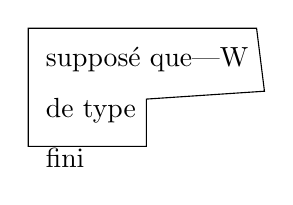
\begin{tikzpicture}[x=1cm,y=1cm]
\node[anchor=west] at (0,1.1) {\unsure{supposé} \unsure{que|W}};
\node[anchor=west] at (0,.45) {\unsure{de type}};
\node[anchor=west] at (0,-.15) {\unsure{fini}};
\draw (-.1,.0)--(-.1,1.5)--(2.8,1.5)--(2.9,.7)--(1.4,.6)--(1.4,.0)--cycle;
\end{tikzpicture}}}

\uline{Théorème 1 bis}
\deleted{Dans le cas $\unsure{\mathrm{II}}$ \unsure{ou} $\unsure{\mathrm I}$, $\mathrm I'$,}
\inserted{Supposons qu'on soit dans le cas $\mathrm I'$.}
\deleted{$\varphi_{S'/S}(\unsure{\mathfrak X})$}
(i) Si $\varphi_{S'/S}(\mathfrak X)$ existe, alors
pour tt ouvert $\mathcal U$ de $\mathfrak X$,
$\varphi_{S'/S}(\mathcal U)$ existe
et $\varphi_{S'/S}(\mathcal U)\to\varphi_{S'/S}(\mathfrak X)$ est une
immersion ouverte.

(ii) Soit $\mathfrak X=\bigcup\mathfrak X_i$, où les $\mathfrak X_i$ sont
tels que pour tt $s\in S$, toute \deleted{\unsure{fibre}}
\inserted{partie finie} de $\mathfrak X_s$ sur $S'_s$ soit contenue dans un $\mathfrak X_i$.
Alors si les $\varphi_{S'/S}(\mathfrak X_i)$ existent, $\varphi_{S'/S}(\mathfrak X)$

\scanpage{76}
% archive foliation: 75
existe et est réunion des $\varphi_{S'/S}(\mathfrak X_i)$.

Démonstration. Il suffit de prouver ii), et pour cela de prouver
que l'hyp. faite implique la condition de recollement. Or,
si $v:T'\to\mathfrak X$ est donné, on introduit les
$T'_i=v^{-1}(\mathfrak X_i)$, \deleted{$\unsure{-}$} et les
\[
T_i=\complement\varphi_T(T'-T'_i),
\]
qui sont des ouverts de $T$, on doit prouver que $T=\bigcup T_i$;
\deleted{et pour ceci, il}
Or $t\in T_i$ signifie que la restriction à $T'_t$ de $\unsure{v|\varphi}$ applique
$T'_t$ dans $\mathfrak X_i$ : donc une section de
$(\mathfrak X_s/S'_s)_{/k(s)}$ définie sur l'extension $k(t)$ de $k(s)$,
doit être contenue dans un des $\mathfrak X_i$.
\margin{\diagram{\begin{tikzcd}[ampersand replacement=\&,column sep=small,row sep=small]
\& \mathfrak X \arrow[d] \\
S \& S' \arrow[l,"\varphi"'] \\
T \arrow[u] \& T' \arrow[l,"\varphi_T"'] \arrow[u,no head] \arrow[uu,bend right=35,dashed,"\unsure{v|u}"']
\end{tikzcd}}}
\margin{\diagram{$\begin{array}{cc}
&\mathfrak X_s\\
k(s)&S'_s\\[1em]
k(t)&T'_t
\end{array}$}}
\deleted{Or \unsure{si on décompose} $S'_s$
\inserted{en des $S_s'^\alpha$}
\unsure{suivant les comp. connexes}
\inserted{$S_s'^\alpha$} $S_s'^\alpha$,
\unsure{on est ramené à} \unsure{ce que chaque} $\alpha$
\unsure{une section de} $\mathfrak X_i^\alpha$ \unsure{sur}}

\uline{Corollaire 1} Si Toute partie \deleted{\unsure{tt}} finie
\inserted{ayant $\leq n(s)$ éléments} d'un $\mathfrak X_s$ est contenue
dans un ouvert affine de $\mathfrak X$, \deleted{alors}
[en particulier si \deleted{$\mathfrak X_s$} \inserted{$\mathfrak X/S$} est
quasi-projectif] alors $\varphi_{S'/S}(\mathfrak X)$ existe, et est
\margin{Soit $n(s)$ le \deleted{\illegible{2}} \unsure{nombre}
\unsure{géom.} \unsure{de points} de $S'/S$}

\scanpage{77}
% archive foliation: 76
réunion des $\varphi_{S'/S}(\mathcal U)$, où $\mathcal U$ parcourt les
ouverts affines de $\mathfrak X$.

\uline{Corollaire 2} Supposons \deleted{de plus}
\inserted{(que tte partie finie de $\mathfrak X$ soit contenue dans un ouvert affine, et)}
$\mathfrak X$ de type fini \inserted{sur $S'$}, et $S$ loc. noeth.
Alors $\varphi_{S'/S}(\mathfrak X)$ est de type fini sur $S$.

La question étant locale \inserted{sur $S$}, on peut supposer $S$ affine.
Tout résulte du

\uline{Lemme} Soit $S$ noethérien, $\mathfrak X$ de type fini sur $S$,
$n$ un entier. \inserted{\deleted{\unsure{les}} $(\mathfrak X_i)_{i\in I}$ famille d'ouverts},
On suppose que tte partie \deleted{finie} $E$ de $\mathfrak X$ telle que
$\operatorname{card}(E)\leq n$ est contenue dans un ouvert
\deleted{\unsure{affine}} $\mathfrak X_i$. Alors il existe une s.-famille finie
de $(\mathfrak X_i)_{i\in I}$ ayant la $=$ propriété.

En effet, l'hyp. signifie que
\[
\bigcup_{i\in I}\underbrace{\mathfrak X_i\times_S-\times_S\mathfrak X_i}_{n\ \text{facteurs}}
=\underbrace{\mathfrak X\times_S-\times_S\mathfrak X}_{n\ \text{facteurs}}.
\]
On applique le fait que $\mathfrak X\times_S\unsure{-}\times_S\mathfrak X$
est \inserted{un espace} noethérien.

\margin{$\unsure{2|\mathcal Z}$ Le foncteur $\underline W^a$ n'est pas local en tous les
\unsure{cas. Car} \illegible{1} il n'existe pas \illegible{1}}

\scanpage{78}
% archive foliation: 77
4) \uline{Application aux immersions, etc}

\uline{Proposition}. Supposons que $\underline W$ soit
\deleted{\unsure{affine} \unsure{spécial} \unsure{de type} $\unsure{\mathrm{II}}$}
\inserted{$\mathrm I'$, ou Greenberg spécial}.
Soit $f:\mathfrak X\to\mathfrak Y$ un morphisme d'immersion
(\deleted{\unsure{ouv.}} fermée).
\inserted{\deleted{loc. de type fini}}
Supposons \deleted{\unsure{en de}} \deleted{\unsure{que}}
dans le cas $\mathrm I'$ que
\inserted{tte partie finie d'un $\mathfrak Y_s$ soit contenue dans un ouvert affine de $\mathfrak Y$.}
\deleted{$\underline W^a(\mathfrak Y)$ existe et est réunion des
$\underline W^a(\mathcal U)$, $\mathcal U$ affines de $\mathfrak Y$.}
\deleted{Alors $\underline W^a(\mathfrak X)$ existe,}
et $\underline W^a(f)$ \inserted{(existe et)} est une immersion fermée.

En effet, on est ramené au cas affine, où cela a été vu.

\uline{Corollaire}
\inserted{(sous les conditions précédentes sur $W$)}
Si $\mathfrak Y$ est quasi-projectif sur $\unsure{S^*|S'}$,
et si $f:\mathfrak X\to\mathfrak Y$ est une immersion,
alors $\underline W^a(f)$ est une immersion.

En effet, $f$ se factorise en
\diagram{\begin{tikzcd}[ampersand replacement=\&]
\mathfrak X \arrow[r,"f'"] \& \mathfrak X' \arrow[r,"f''"] \& \mathfrak Y
\end{tikzcd}}
\deleted{\unsure{imm.}} $f'$ une immers. fermée et $f''$ imm.
ouverte. $\mathfrak X'$ est quasi-projectif \unsure{sur}

\scanpage{79}
% archive foliation: 78
applique la prop. à $f'$, et on applique $=$ à $f''$.

\deleted{\unsure{Prop}} \uline{Corollaire 2}
Sous les conditions de la prop. pour $W$,
\deleted{$\mathfrak X$ \unsure{et}} supposons que
\deleted{$\mathfrak X\unsure{\times}\mathfrak Y$}
tte partie finie de $\mathfrak X$ soit contenue dans un ouvert affine.
Alors si $f:\mathfrak X\to\mathfrak Y$ est séparé, alors il en est
de $=$ de $\underline W^a(f)$ [sous réserve que
$\underline W^a(\mathfrak Y)$ existe dans le cas $\mathrm I'$].

On applique la prop. à $\mathfrak X\unsure{-|\to}\mathfrak X\times_{\mathfrak Y}\mathfrak X$.

\uline{Proposition} $W$, $\mathfrak Y$ comme dans la prop. précédente.
Soit $f:\mathfrak X\to\mathfrak Y$, on suppose
\deleted{$\unsure{\mathfrak X}$ \unsure{quasi}}
\inserted{dans le cas $\mathrm I'$}, pour \unsure{tout} ouvert affine
\inserted{$\mathcal U$} de $\mathfrak Y$,
\inserted{tte partie finie de} $f^{-1}(\mathcal U)$ est
\deleted{\unsure{réunion}} contenue dans un ouvert affine
(p. ex. $f$ quasi-projectif).
On suppose de plus $\mathfrak Y$ loc. noeth et \deleted{$\mathfrak X$}.
$f$ de type fini. \inserted{\deleted{\unsure{resp. affine}}}
Alors $\underline W^a(f)$ est de type fini
\deleted{\unsure{quasi-affine}}.
\margin{\unsure{inquiétude} Dans le cas ``Greenberg spécial'',
\unsure{l'énoncé est} \unsure{valable} \unsure{compte tenu}
\unsure{de la propriété} \unsure{projectif} $\Rightarrow$ quasi-projectif}

\scanpage{80}
% archive foliation: 79
\uline{Proposition} Comme dessus, pour morphismes \uline{affines}.

\scanpage{81}
% archive foliation: 80
\deleted{\uline{\unsure{Notions d'algèbre|Morph. d'algèbres}}\\
\uline{\unsure{multilinéaire|multilinéaires}}}

\uline{Schémas localement}\\
\uline{compacts}

\scanpage{82}
% archive foliation: 81
$Z$ constructible dans $X$ qu. compact,
\inserted{\textcircled{\unsure{ou}}}
\unsure{tt pt} \unsure{a|$\in$} \unsure{un|une} \unsure{syst. fond.|pet. fam.} de \unsure{voisinages rétrocompacts dans} $X$.
\deleted{$Z$ loc. constructible}
\[
\left\{\begin{array}{l}
Z\ \text{qu. cpt et}\\
\forall x\in Z,\ \exists\ \text{un voisinage }U_x\text{ de }x\text{ dans }X,
\text{ tel que }Z\cap U_x\text{ constr. dans }U_x
\end{array}\right.
\]
(alors $\unsure{U}\longrightarrow U'\subset U$, $U'\ni x$, a la $=$ propriété)

nécessité : évident [car $Z$ rétrocompact dans $X$, \deleted{\unsure{dans}}
\unsure{et} on peut prendre $U=X$.

Suffisance. $Z$ est recouvert par un nb fini des $U_x$, soient $U_i$.
Les $U_i\cap Z$ sont constructibles dans $U_i$, donc dans $X$,
donc $Z=\bigcup Z_i$ est constr.

\uline{Corollaire} Supposons $Z$ loc. fermé.
Alors $Z$ \deleted{\unsure{loc.}} constructible
ssi $Z$ est \uline{quasi-compact}, et tt $x\in Z$ a un voisinage ouvert
$U$ dans $X$ tel que $Z\cap U$ soit \uline{fermé} et
\uline{constructible} dans $U$, i.e. $U-Z\cap U$ rétrocompact dans $U$
[i.e. $U-Z\cap U$ quasi-compact,
\inserted{(pour $U$ qu-compact, et si on)}
\unsure{suppose que dans} $X$ l'intersection de deux ouverts quasi-compacts
est qu. cpt)]

\uline{Exemple} Si $X$ est un préschéma quasi-séparé quasi-compact
(p. ex. un schéma quasi-compact, ou un schéma affine) \deleted{\unsure{donc}}
$Z$ loc. fermé dans $X$, alors $Z$ constructible $\Longleftrightarrow$
$Z$ qu. cpt, et tt $x\in Z$ a un voisinage ouvert affine $U$ tel que
$Z\cap U$ \inserted{soit défini par un} \uline{syst. fini} \uline{d'équations}.

% The reversed typewriting showing through this sheet is on the separately supplied reverse, scan 83, where it is transcribed.

\scanpage{83}
% archive foliation: 82
% Printed face of the reused sheet; image rotated 180 degrees for reading.
\begin{center}$-\ 122\ -$\end{center}
\begin{flushright}$n^{\circ}\ 316$\end{flushright}
$V_{(L)}$ est muni canoniquement d'une structure d'espace vectoriel topologique
métrisable et complet (\uline{Esp.} \uline{vect.} \uline{top.} chap. I, § 2, $n^{\circ}3$, th.2).

Soit $(x_p)_{p\in\mathbf Z}$ une famille d'éléments de $V$ tels que $x_p=0$
pour $p$ inférieur à un certain entier rationnel.
Alors la série $\sum_{-\infty}^{+\infty}x_pT^p$ converge dans $V_{(L)}$,
et tout élément de $V_{(L)}$ se met sous cette forme de manière unique.
(Prendre une base dans $V$).

b) L'espace vectoriel $\mathcal L_L(V_{(L)})=(\mathcal L_K(V))_{(L)}$
est muni canoniquement d'une structure d'espace vectoriel topologique métrisable et complet.
Tout endomorphisme de $V_{(L)}$ se met d'une manière unique sous la forme
$\sum_{-\infty}^{+\infty}u_pT^p$, où $u_p\in\mathcal L_K(V)$,
et où les $u_p$ sont nuls pour $p$ inférieur à un certain entier rationnel.

c) Si $K$ est de caractéristique 0, et si $u\in\mathcal L_K(V)$, on pose
$e^{Tu}=1+\frac{1}{1!}uT+\frac{1}{2!}u^2T^2+\cdots\in\mathcal L_L(V_{(L)})$.
Si $x\in V$ est tel que $ux=0$, on a $e^{Tu}.x=x$.

d) Si $W$ est un autre espace vectoriel de dimension finie sur $K$,
et si $v\in\mathcal L_K(W)$, on a
$e^{T(u\otimes1+1\otimes v)}=e^{Tu}\otimes e^{Tv}$.

e) Déduire de c) et d) que, si $V$ est muni d'une structure d'algèbre

\scanpage{84}
% archive foliation: 83
\figure{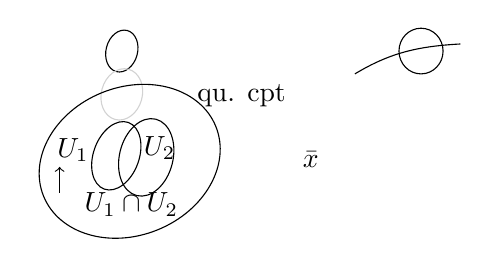
\begin{tikzpicture}[x=1cm,y=1cm]
\draw (-1.05,2.05) ellipse[x radius=.20,y radius=.27,rotate=-15];
\draw[gray!35] (-1.05,1.50) ellipse[x radius=.26,y radius=.33,rotate=-15];
\draw[rotate around={22:(-.95,.65)}] (-.95,.65) ellipse[x radius=1.18,y radius=.94];
\draw[rotate around={-20:(-1.12,.72)}] (-1.12,.72) ellipse[x radius=.29,y radius=.45];
\draw[rotate around={-14:(-.74,.70)}] (-.74,.70) ellipse[x radius=.34,y radius=.50];
\node at (-1.67,.79) {$U_1$};
\node at (-.57,.82) {$U_2$};
\node at (-.93,.10) {$U_1\cap U_2$};
\node at (.47,1.48) {\unsure{qu. cpt}};
\draw[->] (-1.84,.25)--(-1.84,.58);
\node at (1.35,.67) {$\bar x$};
\draw (2.75,2.05) ellipse[x radius=.28,y radius=.29];
\draw (1.91,1.76) .. controls (2.36,2.03) and (2.71,2.11) .. (3.25,2.14);
\end{tikzpicture}}

\figure{\begin{tikzpicture}\draw (0,0)--(6,0);\end{tikzpicture}}
\margin{\figure{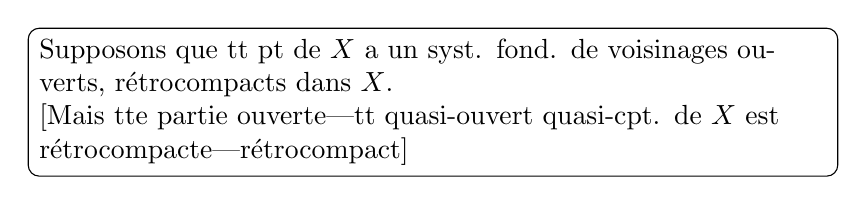
\begin{tikzpicture}
\node[draw,rounded corners=4pt,align=left,text width=10cm,inner sep=4pt] {Supposons que tt pt de $X$ a un syst. fond. de voisinages ouverts,
rétrocompacts dans $X$.\\{}
[Mais \unsure{tte partie ouverte|tt quasi-ouvert} \unsure{quasi-cpt.} de $X$ est \unsure{rétrocompacte|rétrocompact}]};
\end{tikzpicture}}}

Soit $\unsure{F|\mathcal T}$ une partie fermée irréductible de $X$.
Conditions équivalentes
\margin{\diagram{\begin{tikzcd}[ampersand replacement=\&,row sep=small]
\unsure{E} \arrow[d,no head] \\ \unsure{U}
\end{tikzcd}}}

i) Il existe une partie $Z$, ouverte non vide dans $T$,
telle que $Z$ soit constructible dans $X$

ii) Il existe un ouvert \inserted{quasi-compact} $U$ de $X$, tel que
$U\cap T\ne\varnothing$, et $U-U\cap T$ soit qu. cpt.

% Reversed typewriting is show-through from the separately supplied printed face, scan 85.

\scanpage{85}
% archive foliation: 84
% Printed face of the reused sheet; image rotated 180 degrees for reading.
% The upper limit of the initial sum lies beyond the torn edge and is not supplied.
\[
\sum_{j=0}(x_1T_1+\cdots+x_{k-1}T_{k-1})^j x_kT_k
(x_1T_1+\cdots+x_{k-1}T_{k-1})^{k-j-1}
\]
Etant donnés deux éléments $x,y$ de $L$, on définit $g_{i,k-i}(x,y)$ comme
le coefficient de $T_1^iT_2^{k-i}$ dans $(xT_1+yT_2)^k$.
Montrer que l'on a
\[
i!\ (k-i)!\ g_{i,k-i}(x,y)=f_k(t_1,\ldots,t_k)
\]
avec $t_h=x$ pour $h\leq i$ et $t_h=y$ pour $h\geq i+1$.

b) Lorsque $L$ est considérée comme algèbre de Lie sur $K$, on a, dans
$\mathcal L_K(L)$ :
\[
(\operatorname{ad}x)^n=\sum_{i=0}^n(-1)^{n-i}\binom ni L_x^i R_x^{n-i}.
\]
En déduire que, si $K$ est de caractéristique $p$ ($p$ premier), on a :
\[
\begin{aligned}
(1)\qquad &(\operatorname{ad}x)^p.y=(\operatorname{ad}x^p).y\\
(2)\qquad &(\operatorname{ad}x)^{p-1}.y=\sum_{i=0}^{p-1}x^iyx^{p-1-i}
\end{aligned}
\]
Déduire de (2) que :
\[
f_{p-1}(\operatorname{ad}x_1,\ldots,\operatorname{ad}x_{p-1}).y
=f_p(x_1,\ldots,x_{p-1},y)
\]
et :
\[
g_{i,p-1-i}(\operatorname{ad}x,\operatorname{ad}y).y
=(p-i)g_{i,p-i}(x,y).
\]

\scanpage{87}
% archive foliation: 86
\diagram{\begin{tikzcd}[ampersand replacement=\&,row sep=large]
\text{Préschémas atomiques : (réunions de \unsure{spectres|schémas} de corps)}
\arrow[d,"\text{foncteur pleinement fidèle, commutant aux sommes}"']\\
\text{Foncteurs covariants }(\mathrm{Corps})\unsure{-|\to}(\mathrm{Ens})
\end{tikzcd}}
\margin{[Sous-catégorie pleine de $(\mathrm{Sch})$]}
i.e. contravariants $(\text{Schs ponctuels})^\circ\unsure{-|\to}(\mathrm{Ens})$

\diagram{\begin{tikzcd}[ampersand replacement=\&,row sep=large]
\text{Préschémas atomiques sur }k\ [\text{i.e. sur }\operatorname{Spec}(k)]
\arrow[d,"\text{foncteur pleinement fidèle}"']\\
\text{Foncteurs covariants }(\text{Extensions de }k)\unsure{-|\to}(\mathrm{Ens})
\end{tikzcd}}
\margin{$(\mathrm{At})/\operatorname{Spec}k$}
Foncteurs `` '' $(\text{Schs ponctuels}/\operatorname{Spec}k)^\circ\unsure{-|\to}(\mathrm{Ens})$

Soit $X$ un préschéma, il définit un préschéma atomique
\[
|X|=\coprod_{x\in X}\operatorname{Spec}k(x),
\]
qui \deleted{\unsure{est}} \inserted{\unsure{représente}}
la restriction du foncteur contravariant défini par
$X:(\mathrm{Sch})^\circ\unsure{-|\to}(\mathrm{Ens})$,
\deleted{\unsure{aux schémas ponctuels}}.
Bien sûr, on obtient un foncteur $X\mapsto|X|$,
dont la \uline{restriction aux préschémas réduits est fidèle}.
\deleted{\unsure{pleinement}}

Soient $X,Y$ deux préschémas, on appelle \uline{pseudo-morphisme}
ou \uline{application constructible} de $X$ dans $Y$, tt morphisme
$f:|\unsure{\widetilde X|\bar X}|\to|\unsure{\widetilde Y|\bar Y}|$
qui a la propriété suivante : Pour tte partie
\deleted{quasi-compact} \inserted{\unsure{ouvert affine}} $U$ de $X$,
il existe une partition de $U$ en des $U_i$ \inserted{loc. fermés}
(\uline{constructibles}), tels que $f||U_i|$ soit un
\uline{morphisme} $U_{i\,\mathrm{red}}\to Y$.

% Reversed blue typewriting is visible through the reused sheet.

% The reversed typewriting showing through this sheet is on the separately supplied reverse, scan 88, where it is transcribed.

\scanpage{88}
% archive foliation: 87
\begin{center}- 139 -\end{center}
\hfill n\textsuperscript{o} 316

a) Soit $M'_s$ le sous-espace de $M_s$ engendré par les éléments de la forme $\beta_1\otimes\beta_2\otimes\cdots\otimes\beta_s$, où $\beta_i\in\mathcal L(V)$ et où $\beta_i=1$ pour au moins un $i$. Soient $z$ un élément de $U_s$, $z_0=\sum_{1\leq i_1,\ldots,i_s\leq m}a_{i_1\ldots i_s}\alpha_{i_1}\cdots\alpha_{i_s}$ sa composante dans $U^s$, où les $a_{i_1\ldots i_s}$ sont symétriques par rapport aux permutations des indices. Montrer que
\[
\pi_s(z)\equiv s!\sum_{1\leq i_1,\ldots,i_s\leq m}a_{i_1\ldots i_s}\alpha_{i_1}\otimes\cdots\otimes\alpha_{i_s}\quad(\mathrm{mod.}\ M'_s).
\]

b) Déduire de a), que, pour tout $z\in U$, il existe une représentation de dimension finie $\pi$ de $U$ telle que $\pi(z)\neq0$. (Pour une suite de cet exerc., cf.\ §7, exerc.\ 3).

6) - On suppose que $K$ est un corps. Soient $g$ une $K$-algèbre de Lie, $x\longrightarrow x_M$ une représentation de $g$ de dimension finie, $(x_1,\ldots,x_n)$ une base de $M$, et $(x_1^*,\ldots,x_n^*)$ la base duale.

a) Si $f$ est une forme linéaire sur $\overset{r}{\bigotimes}M$, on a :
\[
f=\sum_{1\leq i_1,\ldots,i_r\leq n}f(x_{i_1}\otimes\cdots\otimes x_{i_r})(x_{i_1}^*\otimes\cdots\otimes x_{i_r}^*).
\]

b) Soit $\beta$ une forme bilinéaire non dégénérée sur $M$, invariante pour $g$. Soit $(x'_1,\ldots,x'_n)$ la base de $M$ telle que $\beta(x'_i,x'_j)=\delta_{ij}$. Soit $f$ une forme linéaire invariante sur $\overset{r}{\bigotimes}M$. Déduire de a) que
\[
\sum_{1\leq i_1,\ldots,i_r\leq n}f(x_{i_1}\otimes\cdots\otimes x_{i_r})(x'_{i_1}\otimes\cdots\otimes x'_{i_r})
\]
est un élément invariant de $\overset{r}{\bigotimes}M$ indépendant du choix de la base $(x_i)$.

c) Soit $U$ l'algèbre enveloppante de $g$, $U^*$ l'espace dual de l'espace $U$. La représentation adjointe de $g$ se prolonge en une représentation $x\longrightarrow x_U$ de $g$ dans $U$ définie par $x_Uu=xu-ux$ pour tout $u\in U$. Donc $U^*$ est muni d'une structure de $g$-module. Pour qu'un élément $f$ de $U^*$ soit invariant, il faut et il suffit que $f(uv)=f(vu)$ quels que soient $u,v\in U$.

\scanpage{89}
% archive foliation: 88
\unsure{Transitivité} :
\deleted{[ N.B. il suffit de le vérifier pour des ouverts \deleted{\unsure{aff.}} affines quasi-compacts \inserted{$U^\alpha$} recouvrant $X$, et pour tt $U^\alpha$ \unsure{trouver} un \uline{recouvrement} de $U^\alpha$ par des parties \deleted{constructibles} \inserted{loc. fermées} $U_i^\alpha$, tels que $f\,|\,|U_i^\alpha|$ soit \deleted{\unsure{aff.}} morphisme \ldots}
\margin{$\unsure{\varphi}$}
\margin{\uline{Proposition}}

On appelle \uline{ensemble} \deleted{\unsure{algébrique}}\deleted{\illegible{1}} \uline{schématique} un \deleted{préschéma}, \inserted{préschéma quasi-séparé quasi-compact,} considéré comme objet d'une catégorie dont les morphismes sont les applications constructibles.

\diagram{\begin{tikzcd}[ampersand replacement=\&,column sep=small]
(\mathrm{Sch}\ \deleted{\unsure{\text{réd}}}) \arrow[r] \arrow[rr,bend right=32,"{\deleted{\text{fidèle}}}"'] \arrow[rrr,bend right=48,"{\deleted{\text{fidèle}}}"'] \&
(\mathrm{Sch}) \arrow[r,"{\unsure{\text{n'd}}\ \deleted{\text{fidèle}}}"'] \arrow[rr,bend right=23,"{\deleted{\unsure{\text{fidèle}}}}"'] \&
(\mathrm{ens\ Sch}) \arrow[r,"{\text{fidèle}}"'] \&
(\mathrm{Sch.\ atomes}) \arrow[r,"{\text{pl.\ fid.}}"'] \&
\underline{\mathrm{Hom}}((\mathrm{corps}),\mathrm{Ens})
\end{tikzcd}}

\margin{\figure{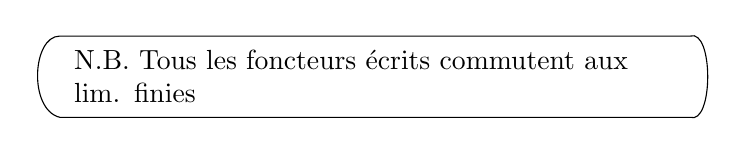
\begin{tikzpicture}
\node[anchor=west,text width=.63\linewidth,inner sep=5pt] (nb) at (0,0) {N.B. \unsure{Tous} les foncteurs écrits commutent aux \unsure{lim.} finies};
\draw (nb.north west) .. controls +(-.35,0) and +(-.4,.1) .. (nb.south west) -- (nb.south east) .. controls +(.3,-.1) and +(.3,.1) .. (nb.north east) -- cycle;
\end{tikzpicture}}}

On s'intéresse \unsure{donc} aux notions sur les ens. schématiques, qui sont invariantes par isom. d'ens schématiques (i.e. isom. constructibles).

Notons $\unsure{\mathfrak S|\mathsection}$ \unsure{comme} \unsure{l.c.q.|l.c.p.}

\diagram{\begin{tikzcd}[ampersand replacement=\&]
X\arrow[r]\&Y\\
X_i\&Y_i\\
X'_j\&\\
X_i\cap X'_j\arrow[r]\&Y_{ij}
\end{tikzcd}}

\uline{Lemme} Soit $X$ préschéma quasi-compact quasi-séparé. \deleted{Alors il existe une} $(Z_i)$ une famille \unsure{quelconque} de parties constructibles recouvrant $X$. Alors il existe une partition de $X$ en des parties loc. fermées constructibles affines, \unsure{plus fine qu'un recouvrement de $X$ par des ens. constructibles}.

\uline{Proposition} Supposons $X$ quasi-séparé et quasi-compact, $f:|X|\longrightarrow|Y|$ donné. Conditions équivalentes

\unsure{a)|i)} $f$ est constructible

\unsure{iii)|ii)} $\exists$ une partition \inserted{finie} de $X$ en des parties \uline{loc. fermées constructibles} $Z_i$, \inserted{\uline{affines}}, telles que $f\,|\,|Z_i|$ soit morphisme

\deleted{\unsure{iii)} Il existe une suite croissante d'ouverts quasi-compacts $U_i$ couvrant $X$, telle que $f\,|\,|U_i-U_{i-1}|$ soit \unsure{morphisme}.}
\figure{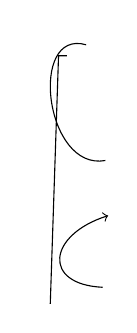
\begin{tikzpicture}[x=.7cm,y=.7cm]
\draw (0,4.5)--(-.15,4.5)--(-.3,0);
\draw (.35,4.7) .. controls (-.7,5) and (-.4,2.4) .. (.7,2.6);
\draw[->] (.65,.3) .. controls (-.45,.35) and (-.35,1.25) .. (.75,1.6);
\end{tikzpicture}}
% The blue reversed typewriting is show-through; its printed face is on scan 90.

\scanpage{90}
% archive foliation: 89
\begin{center}- 138 -\end{center}
\hfill n\textsuperscript{o} 316

dérivation de $V$, alors $s$ et $n$ sont des dérivations de $V$.

4) - On suppose que $K$ est un corps. Soit $g$ une $K$-algèbre de Lie.

a) Soient $x\longrightarrow x_M$ et $x\longrightarrow x_N$ des représentations de $g$, $x\longrightarrow x_N$ étant irréductible et de dimension finie. Soit $(f_j)_{1\leq j\leq n}$ une base de $N$. Si des éléments non tous nuls $e_1,\ldots,e_n$ de $M$ sont tels que $\sum_{i=1}^{n}e_i\otimes f_i$ soit invariant dans $M\otimes N$, alors le sous-espace $M_1$ de $M$ engendré par les $e_i$ est stable pour les $x_M$, et la représentation $x\longrightarrow x_{M_1}$ est duale de la représentation $x\longrightarrow x_N$.

b) Soient $x\longrightarrow x_{M_1}$, $x\longrightarrow x_{M_2}$ deux représentations irréductibles de dimension finie de $g$. Soient $x\longrightarrow x_N$, $x\longrightarrow x_{N^*}$ deux représentations duales de dimension finie de $g$. Pour que le $g$-module $M_1$ soit isomorphe à un sous-$g$-module de $M_2\otimes N$, il faut et il suffit que $M_2$ soit isomorphe à un sous-$g$-module de $M_1\otimes N^*$ (Utiliser a)).

c) Si $M_1$ et $M_2$ sont des \figure{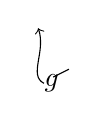
\begin{tikzpicture}[baseline=(g.base)]
\node[inner sep=0pt] (g) at (0,0) {$g$};
\draw[->] (g.west) .. controls +(-.2,.1) and +(.1,-.3) .. (-.17,.7);
\draw (.02,.08)--(.22,.18);
\end{tikzpicture}}-modules simples non isomorphes, et si $K_1$ est une extension de $K$, il n'existe pas de $g_{(K_1)}$-module simple isomorphe à la fois à un sous-$g_{(K_1)}$-module de $M_{1(K_1)}$ et à un sous-$g_{(K_1)}$-module de $M_{2(K_1)}$. (Utiliser a)).

\margin{\P}
5) - On suppose que $K$ est un corps de caractéristique $0$. Soient $V$ un $K$-espace vectoriel de dimension finie, $g=\mathrm{sl}(V)$, $U$ l'algèbre enveloppante de $g$, $U_n$ l'ensemble des éléments de filtration $\leq n$ dans $U$, $U^n$ l'ensemble des éléments symétriques homogènes d'ordre $n$ dans $U$ $(\alpha_1,\ldots,\alpha_m)$ une base de l'espace vectoriel $g$. Soit $W_s=\overset{s}{\bigotimes}V$. La représentation identique de $g$ définit une représentation de $g$ dans $W_s$ qui se prolonge en un homomorphisme $\pi_s$ de $U$ dans l'algèbre $M_s=\mathcal L(W_s)$.

\scanpage{91}
% archive foliation: 90
\uline{Proposition} Soit $f:X-Y$ \deleted{morphisme} application constructible d'ens schématiques. Pour tte partie constructible $E$ de $Y$, $f^{-1}(E)$ est constructible.

\margin{\diagram{\begin{tikzcd}[ampersand replacement=\&]
\deleted{X}\arrow[r]\&\deleted{Y}\\
\deleted{X_i}\arrow[u]\arrow[ur]\&
\end{tikzcd}}}

En effet, soit $X=\coprod_iX_i$, les $X_i$ loc. fermés et constructibles dans $X$, \deleted{Alors} $f_i=(f\,|\,|X_i|)$ un morphisme. On a $f^{-1}(E)=\bigcup f_i^{-1}(\unsure{E_f|E_i})$, il suffit de prouver que chaque $f^{-1}(E)=f^{-1}(E)\cap X_i$ est constructible dans $X$, ou, ce qui revient au même, dans $X_i$ [\deleted{par} par le th. de Chevalley, \inserted{l'immersion} $X_i-X$ étant de présentation finie, pour une structure \unsure{induite} convenable sur $X_i$ \ldots]. Car on se ramène au cas d'un \uline{morphisme} \inserted{\figure{\begin{tikzpicture}[baseline=(p.base)]
\node[draw,ellipse,inner sep=3pt] (p) {\uline{de préschémas}};
\end{tikzpicture}}}, comme il est quasi-compact quasi-séparé c'est connu.

\margin{\unsure{topologique} \unsure{l'argument}\unsure{!}}

\uline{Corollaire} Invariance de la notion de partie constructible d'un ens schématique.

\uline{Proposition} Soit $f:X\longrightarrow Y$ une application constructible de \deleted{ens. schématiques} \inserted{préschémas quasi-compacts quasi-séparés}. Pour que $f$ soit un isom. d'ens schém., il faut et s. qu'il existe \deleted{\unsure{un}} pour un fini $I$, deux partitions $(X_i)_{i\in I}$ et $(Y_j)_{j\in I}$ de $X$ ($Y$) en parties loc. fermées constructibles \inserted{[\unsure{Affines si on veut}]}, telles que $f$ induise un \uline{isom} \uline{de} $X_i$ \uline{sur} $Y_i$.

C'est évidemment suffisant, prouvons la nécessité. Soit $g$ l'inverse de $f$, $X_\alpha,Y_\beta$ deux partitions \inserted{de $X,Y$} mettant en évidence le caractère constructible de $f,g$. \unsure{Évidem.} $f,g$ sont des bijections \unsure{inv.} l'une de l'autre.

\margin{\diagram{\begin{tikzcd}[ampersand replacement=\&]
X\arrow[r,shift left,"f"]\&Y\arrow[l,shift left,"g"]
\end{tikzcd}}}
% The reversed blue typewriting is transcribed on its printed face, scan 92.

\scanpage{92}
% archive foliation: 91
\begin{center}- 137 -\end{center}
\hfill n\textsuperscript{o} 316
\begin{center}- \uline{Exercices sur le §3} -\end{center}

1) - Soient $g$ une algèbre de Lie, $\rho$ une représentation de $g$ dans un $K$-module $M$, $\sigma$ la représentation associée de $g$ dans l'algèbre tensorielle de $M$. Montrer que le sous-module des tenseurs symétriques et le sous-module des tenseurs antisymétriques sont stables pour $\sigma$.

2) - Soient $g$ une algèbre de Lie, $\rho$ une représentation de $g$ dans un $K$-module $M$, $\sigma$ la représentation associée de $g$ dans $Q=\mathcal L(M,M;M)$. Pour qu'un $f\in Q$ soit invariant pour $\sigma$, il faut et il suffit que les $x_M$ soient des dérivations de $M$ muni de la multiplication définie par $f$.

3) - Soit $V$ un espace vectoriel de dimension finie sur un corps parfait $K$.

a) La représentation identique de $\mathrm{gl}(V)$ définit canoniquement des représentations de $\mathrm{gl}(V)$ dans $\overset{p}{\bigotimes}V$ et $\overset{q}{\bigotimes}V^*$, donc une représentation $u\longrightarrow u_q^p$ de $\mathrm{gl}(V)$ dans $V_q^p=(\overset{p}{\bigotimes}V)\otimes(\overset{q}{\bigotimes}V^*)$. Montrer que $u_q^p$ est semi-simple si $u$ l'est. (Se ramener, par extension du corps de base, au cas où $K$ est algébriquement clos). Montrer que $u_q^p$ est nilpotent si $u$ l'est. En déduire que, si $s$ et $n$ sont les composantes semi-simple et nilpotente de $u$, $s_q^p$ et $n_q^p$ sont les composantes semi-simple et nilpotente de $u_q^p$.

b) Déduire de a) que, si un élément de $V_q^p$ est annulé par $u_q^p$, il est annulé par $s_q^p$ et $n_q^p$.

c) Déduire de b) et de l'exerc.2 que, si $V$ est muni d'une structure d'algèbre non nécessairement associative, et si $u$ est une

\scanpage{93}
% archive foliation: 92
Soit $X_{\alpha\beta}=X_\alpha\cap f^{-1}(Y_\beta)$, $Y_{\beta\alpha}=Y_\beta\cap g^{-1}(X_\alpha)$, les $X_{\alpha\beta}$ et $Y_{\beta\alpha}$ sont des ens \uline{constructibles}, qui se correspondent par $f,g$.

\deleted{\unsure{Prenons} \inserted{les} $X_{\alpha\beta}$ \unsure{en une réunion finie} $\bigcup_\lambda X_{\alpha\beta\lambda}$, où $X_{\alpha\beta\lambda}$ est un sous-schéma affine constructible de $X_{\alpha\beta}$ \inserted{\unsure{et de $X_\alpha$}}. Alors $g^{-1}(X_{\alpha\beta\lambda})=g_\beta^{-1}(X_{\alpha\beta\lambda})$ est un sous-schéma de $Y_\beta$ constructible.}

\margin{\diagram{\begin{tikzcd}[ampersand replacement=\&]
X\&Y\\
\&Y_\beta\arrow[ul]
\end{tikzcd}}}

D'ailleurs $X_{\alpha\beta}=f_\alpha^{-1}(Y_\beta)$ est un \deleted{sous-schéma de} loc. fermé dans $X_\alpha$, donc dans $X$. Et $f_{\alpha\beta}:X_{\alpha\beta}\longrightarrow Y$ est un morphisme \inserted{de schémas} (car induit par $f_\alpha:X_\alpha\longrightarrow Y$]. \deleted{\unsure{Donc il est}} De même, les $Y_{\alpha\beta}$ sont constructibles et loc. fermés, et \inserted{$g_{\alpha\beta}:Y_{\alpha\beta}\longrightarrow X$ est un morphisme de schém.}

Enfin \deleted{comme} $X_{\alpha\beta}\longrightarrow Y_\beta$ se factorise par un \unsure{morph.} $X_{\alpha\beta}\longrightarrow Y_{\alpha\beta}$ [car il le fait ens.], et de même on a un \uline{morphisme} $Y_{\alpha\beta}\longrightarrow X_{\alpha\beta}$. Ces derniers sont donc inverses l'un de l'autre.

\uline{Cor. 0} Si $X$ noethérien $Y$ l'est.

\uline{Cor. 1} Tout ens schématique est isomorphe à un $|X|$, pour $X$ affine.

\uline{Cor. 2} Tout morphisme d'ens schématiques est isom. à un morphisme de \deleted{\unsure{ens}} schémas affines. (Considéré comme application constructible).

Démonstration et remarque.

\margin{\figure{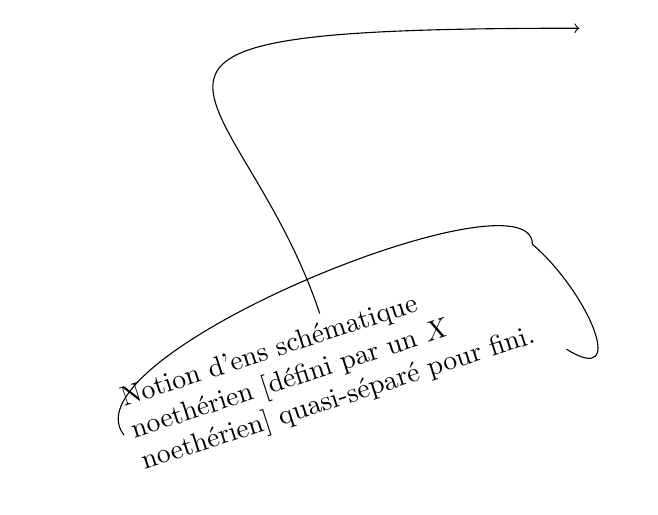
\begin{tikzpicture}
\node[anchor=north west,text width=.45\linewidth,inner sep=3pt,rotate=18] (n) at (0,0) {\uline{Notion} d'ens \unsure{schématique} \uline{noethérien} [\unsure{défini par} \unsure{un} $X$ \unsure{noethérien}] \unsure{quasi-séparé} \unsure{pour} \unsure{fini}.};
\draw[->] (n.north) .. controls +(-1,3) and +(-7,0) .. (6,4.5);
\draw (n.west) .. controls +(-.8,1) and +(0,1) .. (n.north east) .. controls +(.7,-.6) and +(.8,-.5) .. (n.south east);
\end{tikzpicture}}}

\uline{Cor. 3} Un \deleted{isom} \inserted{morphisme $f:X\longrightarrow Y$} de préschémas quasi-compacts et quasi-séparés qui est un isom d'ens schématiques est \uline{de type fini}.
% Reversed blue typewriting is transcribed on its printed face, scan 94.

\scanpage{94}
% archive foliation: 93
\begin{center}- 37 -\end{center}
\hfill n\textsuperscript{o} 288

dont les projections sur les facteurs $E_i$ sont bornées, que les parties bornées de $E_i$ sont contenues (du moins si $K$ est non discret) dans un homothétique de la boule unité de $E_i$, il s'ensuit aisément que sur l'espace vectoriel $L(E_1,\ldots,E_n\,;\,F)$, la topologie de la convergence bornée est définie par l'unique norme :
\[
\|u\|=\operatorname{Sup}\|u(x_1,\ldots,x_n)\|\quad\text{pour}\quad\|x_1\|<1,\ldots,\|x_n\|\leq1
\]
Ceci mérite sans doute une proposition en forme et une rédaction moins cursive, mais l'endroit pour ces sorites semblerait plutôt dans les E.V.T.

\scanpage{95}
% archive foliation: 94
\uline{Morphisme de type fini} \deleted{\inserted{[\unsure{prés. finie|quasi-fini}]}} d'ens schématiques : tel qu'il existe une partition de $X$ en ensembles loc. fermés constructibles affines $X_i$, telle que les $f\,|\,X_i$ soient des morphismes de type fini \deleted{[\unsure{prés. finie|quasi-fini}]}.

\margin{\unsure{cela implique} \unsure{la définition} \unsure{présentation finie} ?}

Un tel morphisme d'ens schématique est isom. à un morphisme de type fini de schémas affines, (considéré comme morphisme d'ens schématiques). \uline{Transitivité}.

Ens. schématique sur un autre, de type fini sur un autre. Tous sont sur $\unsure{\mathbf Z|Z}$ !

Ens. schématique défini par une partie constructible d'un ens. schématique, son immersion canonique, décomposition de $X$ en somme $X=E\amalg(X-E)$, critère de factorisabilité par une partie constructible; \uline{universalité} !

Produit fibré [et $\varprojlim$ finies] dans la catégorie des ens schématiques. \uline{Existe}, et le foncteur \deleted{préschémas}
\diagram{\begin{tikzcd}[ampersand replacement=\&]
(\text{présch qu compt qu sép})\arrow[r]\&(\text{ens schém})
\end{tikzcd}}
commute aux produits fibrés.

Si on a $X$ et $Y$ sur $Z$, si $X',Y'$ sont des parties constructibles de $X,Y$ alors
\[
X'\times_ZY'=\operatorname{pr}_1^{-1}(X')\cap\operatorname{pr}_2^{-1}(Y')\quad\ldots.
\]
% Reversed blue typewriting is transcribed on its printed face, scan 96.

\scanpage{96}
% archive foliation: 95
\hfill n\textsuperscript{o} 285
\begin{center}
RAPPORT sur la RÉÉDITION\\
de\\
TOPOLOGIE GENERALE\\
Chap.III
\end{center}

§2 ; les n\textsuperscript{os} 4 et 8 sont remaniés de la façon suivante :

4. - \uline{Espaces homogènes}

Soient $E$ un espace topologique, $G$ un groupe topologique, et supposons $E$ muni du groupe d'opérateurs $G$ (Alg. chap.I, §7, n\textsuperscript{o}2) ; nous dirons que $G$ \uline{opère continûment} dans $E$ si l'application $(s,x)\longrightarrow s.x$ de $G\times E$ dans $E$ est \uline{continue}. Lorsqu'il en est ainsi, pour tout $s\in G$, l'application $x\longrightarrow s.x$ de $E$ dans $E$ est un \uline{homéomorphisme} de $E$ sur lui-même, car c'est une bijection continue dont la bijection réciproque $x\longrightarrow s^{-1}.x$ est aussi continue.

Supposons en outre que $G$ opère \uline{transitivement} dans $E$, autrement dit que $E$ soit (au sens algébrique) un \uline{espace homogène} de $G$ (Alg., chap.I, §7,n\textsuperscript{o}6). Soient $x_{\unsure{o|0}}$ un point de $E$, $H_{\unsure{o|0}}$ le sous-groupe de $G$ formé des opérateurs laissant invariant $x_{\unsure{o|0}}$ ( en \uline{Alg.}, Bourbaki n'a pas cru bon de donner un nom à ce sous-groupe ; faut-il rattraper cela, et l'appeler ``stabilisateur'' de $x_{\unsure{o|0}}$ ?). La surjection continue $s\longrightarrow s.x_{\unsure{o|0}}$ de $G$ sur $E$ se factorise canoniquement en
\diagram{\begin{tikzcd}[ampersand replacement=\&]
G\arrow[r,"f"]\&G/H_{\unsure{o|0}}\arrow[r,"g"]\&E
\end{tikzcd}}
où $f$ est l'application canonique de $G$ sur l'espace homogène $G/H_{\unsure{o|0}}$ et $g$ la bijection $s.H_{\unsure{o|0}}\longrightarrow s.x_{\unsure{o|0}}$ de $G/H_{\unsure{o|0}}$ sur $E$ ; on sait en outre (Chap.I, 2\textsuperscript{eme} éd. §9, n\textsuperscript{o}2, th.1) que si on munit $G/H_{\unsure{o|0}}$ de la topologie quotient de celle de $G$ par la relation d'équivalence $s^{-1}t\in H_{\unsure{o|0}}$, $g$ est \uline{continue}. On dit que $E$ est un \uline{espace homogène topologique}(correspondant

\scanpage{97}
% archive foliation: 96
$(X_i)_{i\in I}$ système projectif filtrant de préschémas quasi-compacts quasi-séparés,
\[
\exists i\quad\text{tq.}\quad j\geq i\Longrightarrow u_{ij}\text{ est affine}.
\]
Donc $X=\varprojlim X_i$ existe.

\deleted{Je dis que} \inserted{A-t-on}
\[
\operatorname{cons}X\xrightarrow{\sim}\varprojlim\operatorname{cons}(X_i)\qquad ???
\]

En effet, soit $T$ un préschéma quasi-compact et quasi-séparé, alors on a
\[
\operatorname{Hom}(\operatorname{cons}T,\operatorname{cons}X)
=\operatorname{App\,cons}(T,X)
=\varinjlim_{\substack{\beta\ \text{une}\\\text{partition finie de}\\T\ \text{en ens. loc.}\\\text{fermés constructibles}}}
\operatorname{Hom}\left(\deleted{\unsure{T_1|T_i}}\coprod_{\alpha\in\operatorname{Ind}(\beta)}T_{\unsure{i|\alpha}}^\beta,X\right)
\]
\[
=\varinjlim_\beta\varprojlim_i\prod_{\alpha\in\operatorname{Ind}(\beta)}\operatorname{Hom}(T_\alpha^\beta,X_i)
\]
\[
\operatorname{Hom}\left(\operatorname{cons}(T),\deleted{\unsure{\operatorname{cons}X}}\varprojlim_i\operatorname{cons}(X_i)\right)
=\varprojlim_i\varinjlim_\beta\prod_{\alpha\in\operatorname{Ind}\beta}\operatorname{Hom}(T_\alpha^\beta,X_i)
\]

Cependant, considérons un sch affine comme $X$, un $(Y_j)_{j\in J}$, d'où
\[
Y=\varprojlim Y_j
\]
quels sont les \deleted{morphismes} appl. constructibles de $X$ dans $Y$ ? \deleted{Il faut d'abord}
\[
\operatorname{Hom}(\operatorname{cons}X,\operatorname{cons}Y)
=\varinjlim_{\substack{\beta\ \text{partitions}\\\text{finies de}\\X\ \text{en parties loc.}\\\text{fermées constr.}\ X_\alpha^\beta}}
\prod_\alpha\operatorname{Hom}(\deleted{\unsure{\coprod_\beta|\sum_\beta}}X_\alpha^\beta,Y)
\]
% Reversed blue typewriting is transcribed on its printed face, scan 98.

\scanpage{98}
% archive foliation: 97
\begin{center}- 13 -\end{center}
\hfill n\textsuperscript{o} 285

formée de sous-groupes distingués fermés de $G$, et qui converge vers $e$; en outre, lorsque les conditions de la prop.24 sont satisfaites, $G_\alpha$ est isomorphe à $G/N_\alpha$. Inversement :

PROPOSITION 25 - \uline{Soient} $G$ \uline{un groupe topologique séparé}, $(H_\alpha)$ \uline{une base de filtre sur} $E$, \uline{formée de sous-groupes distingués fermés et convergente vers} $e$. \uline{Pour} $H_\beta\subset H_\alpha$, \uline{soit} $f_{\alpha\beta}$ \uline{l'application canonique de} $G/H_\beta$ \uline{sur} $G/H_\alpha$ ; \uline{alors} $(G/H_\alpha,f_{\alpha\beta})$ \uline{est un système projectif de groupes topologiques vérifiant les conditions de la prop.24}, \uline{et si} $g_\alpha$ \uline{est l'application canonique de} $G$ \uline{sur} $G/H_\alpha$, $g=(g_\alpha)$ \uline{est un isomorphisme de} $G$ \uline{sur un sous-groupe partout dense de} $G'=\varprojlim G/H_\alpha$.

Pour $H_\beta\subset H_\alpha$,(relation de préordre que l'on notera $\alpha\leq\beta$), $G/H_\alpha$ s'identifie canoniquement à $(G/H_\beta)/(H_\alpha/H_\beta)$ (prop.16), donc $f_{\alpha\beta}$ est un homomorphisme, et il est immédiat que si $\alpha\leq\beta\leq\gamma$, $f_{\alpha\beta}\circ f_{\beta\gamma}=f_{\alpha\gamma}$. En outre on a, pour $H_\beta\subset H_\alpha$, $g_\alpha=f_{\alpha\beta}\circ g_\beta$, donc $g$ est une représentation continue de $G$ dans $G'$ (prop.20), et comme l'intersection des $H_\alpha$ est réduite à $e$, $g$ est injective. Comme $g_\alpha$ est surjective, il en est de même de l'application canonique de $G'$ sur $G/H_\alpha$; la prop.24 montre en outre que $g(G)$ est partout dense dans $G'$. Enfin, soit $V$ un voisinage de $e$ dans $G$, et soit $\alpha$ un indice tel que $H_\alpha\subset V$ ; l'ensemble des $y'=g(y)$ tels que $g_\alpha(y)\in g_\alpha(V)$ est un voisinage $W$ de l'élément neutre dans le sous-groupe $g(G)$ de $G'$. Mais la relation $g_\alpha(y)\in g_\alpha(V)$ entraîne par définition $y\in VH_\alpha\subset V^2$ ; on voit donc que $g(V^2)$ est un voisinage de l'élément neutre dans $g(G)$, ce qui achève la démonstration.

On dit que $g$ est \uline{l'application canonique} de $G$ dans $G'=\varprojlim G/H_\alpha$.

On notera que l'on n'a pas nécessairement $g(G)=G'$ (exerc).
